%! suppress = MissingLabel

Продолжения с начала 60х не один раз возникали в литературе в различных формах и разнообразных приложениях~\cite{reynolds1993discoveries, landin1997histories}, пока в 70х Wadsworth не придумал общий термин и единую концепцию --- \vocab{continuation}\footnote{\url{https://en.wikipedia.org/wiki/Continuation}} --- ``the meaning of the rest of the program''.

Начальным толчком к размышлениям стал язык Algol 60, имевший нетривиальный механизм меток и прыжков.
Проблемой была как имплементация семантики, так и её денотационное описание вместе с трансляцией в лямбда-исчисление.
Действительно, как математически описать \texttt{goto}?
В каком домене искать семантику таких программ?
Как написать определяющий интерпретатор, отправляющий программу в этот домен?
Решением стала возможность сослаться на семантику остатка программы, продолжение, в определённой точке (например, на метке).

Если мы внимательно рассмотрим процесс вычисления выражений, мы обнаружим, что он состоит из двух этапов: поиска подвыражения (редекса), в котором можно сделать элементарный шаг вычислений, выполнение этого шага, и так далее\footnote{На самом деле вычислениям с продолжениями учат в начальных классах, когда рассказывают про вычисление выражений ``по действиям''.}.
Во время поиска редекса, выражение разбивается на две части (см.~\ref{fig:basic-continuation}):
\begin{itemize}
    \item Фокус --- подвыражение в котором ищем редекс;
    \item Продолжение --- остаток выражения с ``дыркой'', обозначающий место, куда нужно подставить результат шага вычислений.
\end{itemize}

\begin{figure}[h]
    \centering
    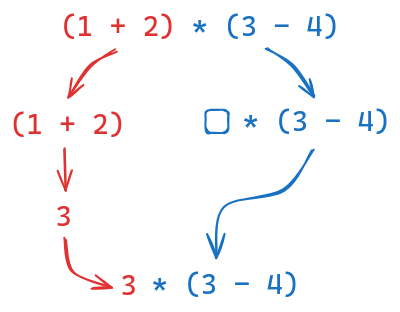
\includegraphics[width=0.35\textwidth]{figs/cont-expr}
    \caption{Выражение разделяется на фокус (красный) и продолжение (синее), когда в фокусе удалось сделать шаг, они объединяются в новое выражение, для которого процесс повторяется.}
    \label{fig:basic-continuation}
\end{figure}

Как правило, продолжения существуют вне пользовательского кода как состояние интерпретатора, которому нужно помнить, что и как исполнять дальше в каждый момент времени.
Однако, языки предоставляют пользователям множество конструкций, позволяющих управлять продолжениями:

\begin{itemize}
    \item Функция \mintinline{kotlin}|exit| выбрасывает продолжение программы целиком;
    \item Конструкция \mintinline{kotlin}|try-catch| позволяет выбросить часть продолжения до места поимки исключения и восстановить доставшееся;
    \item Конструкция \mintinline{kotlin}|return| позволяет восстановить исполнение в месте, где функция была вызвана;
    \item Конструкции \mintinline{kotlin}|break| и \mintinline{kotlin}|continue| восстанавливают продолжение после цикла и до\ldots
\end{itemize}

\begin{figure}[h]
    \centering
    \begin{subfigure}[h]{0.29\linewidth}
        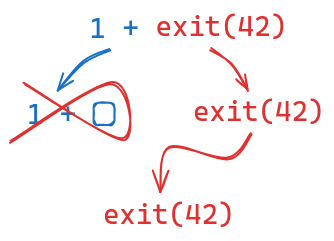
\includegraphics[width=1\textwidth]{figs/cont-exit}
    \end{subfigure}
    \begin{subfigure}[h]{0.7\linewidth}
        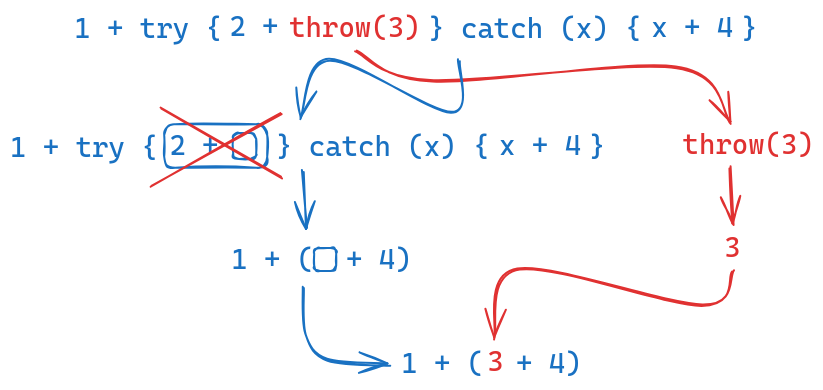
\includegraphics[width=1\textwidth]{figs/cont-try-catch}
    \end{subfigure}
\end{figure}

В примерах выше конструкции языка управляют продолжениями неявно.
Однако, иногда вводят операторы, позволяющие явно оперировать продолжениями.

\vocab{Продолжения первого класса (first-class continuations)} --- продолжения, которые представимы в программе в виде значений.
Учитывая, что продолжение имеет вакантное место ещё не вычисленного подвыражения, продолжения первого класса представляют функциями первого класса.

Чтобы получить в коде продолжение первого класса, нужно либо написать код в специальном виде, либо воспользоваться встроенным в язык оператором~\cite[приложение A]{hillerstrom2022foundations}.
Например, $J$, \texttt{escape}~\cite{reynolds1972definitional}, \texttt{call/cc}\ldots % todo ref CPS

\subsection{Continuation semantics} \label{subsec:definctionalized-cont}

Как обычно, следуя Hutton's Razor, рассмотрим интерпретацию маленького простого язычка с вычитанием (несимметричная операция для проверки реализации):
\begin{minted}{haskell}
    data Expr = Const Int | Diff Expr Expr

    eval :: Expr -> Int
    eval = \case Const x -> x; Diff l r -> eval l - eval r
\end{minted}

Перепишем этот интерпретатор в стиле с явными продолжениями, явно выделяя шаги поиска элементарных подвыражений.

% todo reduction semantics, plt redex

\subsubsection{Прямолинейная реализация}

Заведём структуру данных, буквально соответствующую ``выражению с дыркой''.
Заметьте, что тут мы уже однозначно фиксируем порядок вычисления операндов.
\begin{minted}{haskell}
    data K
      = Hole         -- дырка ?$\boxempty$?
      | LDiff K Expr -- фокус пошел в правое подвыражение, запомнили левое
      | RDiff Int K  -- посчитали левое, фокус пошел вправо
\end{minted}

По мере того как мы спускаемся вглубь фокуса, нам нужно уметь наращивать продолжение, подставляя новый кусочек вместо дырки:
\begin{minted}{haskell}
    substHole :: K -> K -> K
    substHole to target = case to of
      Hole -> target
      LDiff to' r -> LDiff (to' `substHole` target) r
      RDiff l to' -> RDiff l (to' `substHole` target)
\end{minted}

Теперь напишем интерпретатор в виде двух взаиморекурсивных функций:
\begin{minted}{haskell}
    evalK :: Expr -> K -> Int
    evalK expr k = case expr of
      Const x -> k `appK` x
      Diff l r ->
        let k' = k `substHole` LDiff Hole r in -- запоминаем, что пошли влево
        evalK l k'                             -- идём влево

    appK :: K -> Int -> Int
    appK k result = case k of
      Hole -> result
      LDiff k' r ->
        let result' = k' `appK` result in -- довычисляем левое подвыражение
        evalK r (RDiff result' Hole)      -- идём вправо, запомнив результат слева
      RDiff l k' -> l - k' `appK` result  -- наконец-то вычисляем минус
\end{minted}

Выражение можно вычислить, запустив \texttt{evalK} на пустом продолжении \mintinline{haskell}{Hole}.

Заметим, что \mintinline{haskell}{K} вместе с \texttt{appK} представляют собой набор дефункционализированных замыканий.
Вернёмся к этому далее. % todo ref

\subsubsection{Продолжение как стек}

Перепишем структуру данных \mintinline{haskell}{K} эквивалентным образом (см~\ref{subsec:recursive-types}):
\[
    \begin{array}{l}
        K = 1 + K \times Expr + Int \times K \\
        K = 1 + (Expr + Int) \times K
    \end{array}
\]
Так, продолжение можно представить в виде функционального списка фреймов:
\begin{minted}{haskell}
    data Frame = LDiff Expr | RDiff Int
    type K = [Frame]
\end{minted}
Новые фреймы будем добавлять не в конец, как мы делали ранее, а в начало:
\begin{minted}{haskell}
    evalK :: Expr -> K -> Int
    evalK expr k = case expr of
      Const x -> k `appK` x
      Diff l r -> eval l (LDiff r : k)

    appK :: K -> Int -> Int
    appK k result = case k of
      [] -> result
      LDiff r : k' -> evalK r (RDiff result : k')
      RDiff l : k' -> k' `appK` (l - result)
\end{minted}

Таким образом, мы представили продолжение в виде стека.
На самом деле аппаратный стек как раз и выполняет роль продолжения (вместе с регистрами).

% todo calculating correct compilers








%\begin{figure}
%    \centering
%    \begin{tabular}{|c|c|}
%        \hline
%        Фокус         & Продолжение           \\
%        \hline
%        $(5 - 2) - 1$ & $\boxempty$           \\
%        $5 - 2$       & $\boxempty - 1$       \\
%        $5$           & $(\boxempty - 2) - 1$ \\
%        $2$           & $(5 - \boxempty) - 1$ \\
%        $2$           & $(5 - \boxempty) - 1$ \\
%        \hline
%    \end{tabular}
%\end{figure}

%\subsection{Continuation-passing style (CPS)}
%
%% todo higher-order CPS
%
%Базовым способом получить в программе продолжение первого класса --- написать программу в CPS.
%CPS эксплуатирует следующий изоморфизм:
%\begin{minted}{haskell}
%    to :: a -> (forall r . (a -> r) -> r)
%    to x k = k x
%
%    from :: (forall r . (a -> r) -> r) -> a
%    from comp = comp id
%\end{minted}
%
%Иначе говоря, вместо того, чтобы предоставить значение, можно запросить у вызывающей стороны, как она собирается с этим значением работать, сделать это самостоятельно и вернуть вызывающей стороне\footnote{\url{https://wiki.haskell.org/Cont_computations_as_question-answering_boxes}}.
%
%% todo yoneda lemma
%
%Корни этого изоморфизма в лемме Йонеды из теории категорий~\cite{hinze2010reason}.
%Прикладным же программистам он знаком по технике использования callback'ов.
%
%Например, мы можем переписать факториал в стиле CPS.
%Заметьте, что код имеет доступ к продолжению первого класса (однако, никак нетривиально не использует его).
%\begin{minted}{haskell}
%    facCps :: Int -> (forall r . (Int -> r) -> r)
%    facCps n k
%      | n <= 1 = k 1
%      | otherwise = facCps (n - 1) \res -> k (n * res)
%\end{minted}
%
%\begin{task}
%    Вручную поредуцируйте определение \mintinline{haskell}|facCps| на простом примере.
%\end{task}
%
%\begin{task}
%    Сколько функция \mintinline{haskell}|facCps| потребляет стековой памяти?
%\end{task}
%
%\subsubsection{Монада \texttt{Cont}}
%
%Из-за CPS код потерял привычную структуру, при которой функции напрямую возвращают свои результаты (i.e. \vocab{direct style}).
%При наличии большого количества вызовов трансформированных функций, код становится плохо читаемым.
%
%\begin{minted}{haskell}
%    fibCps :: Int -> (forall r . (Int -> r) -> r)
%    fibCps n k = if n <= 2 then k 1 else
%      fibCps (n - 1) \res1 ->
%      fibCps (n - 2) \res2 ->
%      k (res1 + res2)
%\end{minted}
%
%Однако, можно заметить, что монадическое связывание вторым аргументом тоже принимает продолжение, но ``маленькое'', до конца \mintinline{haskell}|do|-блока.
%Таким образом, можно попробовать линеаризовать CPS код с помощью монад.
%
%Заведём \mintinline{haskell}|newtype| обёртку для объявления инстансов:
%\begin{minted}{haskell}
%    newtype Cont r a = Cont { runCont :: (a -> r) -> r }
%\end{minted}
%
%Функтор добавляет пост-процессинг результату перед передачей в продолжение:
%\begin{minted}{haskell}
%    instance Functor (Cont r) where
%      -- fmap :: (a -> b) -> ((a -> r) -> r) -> ((b -> r) -> r)
%      fmap f (Cont comp) = Cont \k -> comp (k . f)
%\end{minted}
%
%Аппликатив просто передаёт значение продолжению:
%\begin{minted}{haskell}
%    instance Applicative (Cont r) where
%      pure x = Cont \k -> k x
%      (<*>) = ap
%\end{minted}
%
%Наконец, монада принимает в связывании ``маленькое'' продолжение, композирует его с ``большим'' продолжением, пришедшим снаружи, и передаёт в данное вычисление:
%\begin{minted}{haskell}
%    instance Monad (Cont r) where
%      Cont comp >>= k = Cont \k' -> comp \x -> runCont (k x) k'
%\end{minted}
%
%Теперь мы можем писать линейный код, а монадическая машинерия сама конструирует продолжения и подкладывает в предыдущие вычисления:
%\begin{minted}{haskell}
%    fibCont :: Int -> Cont r Int
%    fibCont n = if n <= 2 then pure 1 else do
%      res1 <- fibCont (n - 1)
%      res2 <- fibCont (n - 2)
%      pure (res1 + res2)
%\end{minted}
%
%\begin{task}
%    Оборвите вычисление, если \texttt{res1} больше \texttt{50}.
%\end{task}
%
%\begin{task}
%    Оборвите вычисление как только общий результат стал больше 50.
%\end{task}
%
%\subsubsection{\texttt{call/cc}}
%
%Можно получить доступ к продолжению просто написав где-то в \mintinline{haskell}|do|-нотации конструктор:
%\begin{minted}{haskell}
%    do ...; Cont \?\framebox{k}? -> ...; ...
%\end{minted}
%Однако, для получения продолжений, как правило, пользуются специальными операторами.
%Классическим примером является \texttt{call/cc} (call with current continuation):
%\begin{minted}{haskell}
%    callCC :: ((a -> Cont r b) -> Cont r a) -> Cont r a
%    callCC f = Cont \k -> runCont (f \x -> Cont \_ -> k x) k
%\end{minted}
%
%\texttt{call/cc} принимает функцию \texttt{f}, в которую передаёт текущее продолжение (рис.~\ref{fig:call-cc}).
%При этом вызов продолжения работает как \mintinline{kotlin}|return| для \texttt{f} (продолжение не содержит кода \texttt{f}):
%\begin{minted}{haskell}
%    foo :: Int -> Cont r String
%    foo x = callCC $ \k -> do
%      let y = x ^ 2 + 3
%      when (y > 20) $ k "over twenty"
%      return (show $ y - 4)
%\end{minted}
%
%\begin{figure}[h]
%    \centering
%    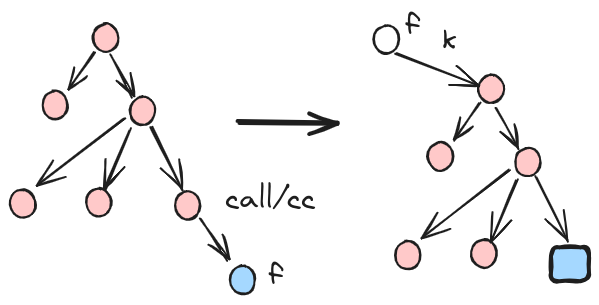
\includegraphics[width=0.6\linewidth]{figs/call-cc}
%    \caption{\texttt{call/cc} вызывает функцию \texttt{f} с продолжением \texttt{k}.
%    Аргумент \texttt{k} (или результат \texttt{f}) подставляется вместо вхождения \texttt{call/cc}.}
%    \label{fig:call-cc}
%\end{figure}
%
%Например, с помощью \texttt{call/cc} можно реализовать кооперативную многозадачность\footnote{\href{https://en.wikibooks.org/wiki/Haskell/Continuation_passing_style\#Example:_coroutines}{(wiki) Continuation-passing style.
%Example: coroutines.}}.
%Однако, считается, что \texttt{call/cc} --- не самый удачный примитив\footnote{\url{https://okmij.org/ftp/continuations/against-callcc.html}}.
%
%\subsubsection{Continuation semantics}
%
%Существует стиль формальных семантики, называемый \vocab{continuation semantics}.
%Фактически он соответствует написанию определяющих интерпретаторов в CPS\footnote{\url{https://ncatlab.org/nlab/show/continuation-passing+style}}.
%CPS эксплицирует продолжения, иначе они были бы полностью в ведении какого-нибудь более базового интерпретатора в башне.
%
%Заметьте, что то, что мы строили выше, является shallow embedding некоторого языка, заданного в continuation semantics.
%Реализация интерпретатора для deep embedding из~\ref{subsubsec:h-syntax}, например, будет выглядеть следующим образом:
%\begin{minted}{haskell}
%    eval3' :: Term3 ty -> (forall r . (ty -> Maybe r) -> Maybe r)
%    eval3' term k = case term of
%      Val3 x -> k x
%      Plus l r -> eval3' l \l' -> eval3' r \r' -> k (l' + r')
%      App3 f arg -> eval3' f \f' -> eval3' arg \arg' -> k (f' arg')
%      Lam3 f -> k \arg -> eval3' (f (Val3 arg)) id
%      Abort -> Nothing
%\end{minted}
%
%Язык с CPS интерпретатором расширить управляющими конструкциями вроде \texttt{call/cc}.
%Также можно заметить, что реализация интерпретатора стала хвостово-рекурсивной, а стратегии больше не определяется мета-языком~\cite{reynolds1972definitional}.
%
%% todo call/cc
%
%Проследить семантику операций также можно в следующей нотации, эксплицирующей продолжения:
%
%\begin{align*}
%    E[abort(e)] &\rightsquigarrow e\\
%    E[call/cc(f)] &\rightsquigarrow E[f(\lambda x\ldotp E[x])]
%\end{align*}
%
%\subsubsection{Эффективный CPS}
%
%В нашей реализации CPS производится огромное количество аллокаций замыканий, реифицирующих продолжения.
%Однако, если CPS получается автоматической трансляцией, можно делать эффективнее.
%Изначально продолжения придумывались для описания семантики прыжков, но можно пойти и в обратную сторону, реализовав продолжения эффективно для современных машин через \texttt{goto}.
%
%Так, состояние функции целиком один раз аллоцируется в куче, а перемещения по телу реализованы как машина состояний --- с помощью меток и прыжков.
%Таким образом, например, реализованы безстековые корутины в Kotlin\footnote{\url{https://github.com/Kotlin/KEEP/blob/master/proposals/coroutines.md\#state-machines} \label{note:kotlin-state}}, генераторы в C\#\footnote{\url{https://csharpindepth.com/Articles/IteratorBlockImplementation}}\ldots
%
%Даже в таком виде CPS остаётся тяжеловесной трансформацией, способной замедлить исполнение кода на порядки.
%Дело, в частности, в том, что переменные в таком подходе сложно размещать в регистрах (у функций много точек выходов и входов\footref{note:kotlin-state}), приходится постоянно записывать их в RAM --- производить spilling\footnote{\url{https://en.wikipedia.org/wiki/Register_allocation}}.
%
%% todo объяснение через дефункционализацию
%
%% todo move to implementation section
%
%%\subsection{Дефункционализация продолжений}
%%
%%\cite{ager2003functional, huet1997zipper, mcbride2001derivative}
%%
%%\footnote{\url{https://ncatlab.org/nlab/show/defunctionalization}}
%%
%%\cite{reynolds1972definitional}
%
%% todo link to youtube
%
%% todo zipper and nested continuations
%
%% todo huet zipper
%
%% todo zipper context and derivations
%
%% todo abstract machines
%
%% todo
%
%\subsection{Delimited continuations}
%
%Ранее мы рассматривали \vocab{неограниченные (undelimited) продолжения}, которые представляют собой весь остаток программы до её конца.
%В том числе, мы рассматривали оператор \texttt{call/cc}, который реифицирует неограниченное продолжение в виде функции для непосредственного использования пользователем.
%Однако, предоставление пользователю неограниченных продолжений ведёт к множеству проблем и не очень полезно на практике~\footnote{\url{https://okmij.org/ftp/continuations/against-callcc.html}}.
%
%Более того, неограниченные продолжения де-факто --- не совсем функции, так как они не возвращают результата (он уже ``beyond the grave''), следовательно, они также не композируются (как и странно композировать \texttt{abort} с \texttt{exit})\footnote{\url{https://okmij.org/ftp/continuations/undelimited.html}}.
%Неограниченные продолжения --- это скорее ко-значения, пока часть программы выполняется, они ожидают её результата~\cite{curien2000duality}.
%
%Вместо этого вводятся парные операторы для работы с \vocab{ограниченными (delimited) продолжениями}\footnote{\url{https://www.cl.cam.ac.uk/teaching/2324/R277/handout-delimited-continuations.pdf}}\footnote{\href{https://youtu.be/TE48LsgVlIU?si=cBdUCzYwYWpwPkkh}{(youtube)  Keynote: Delimited Continuations, Demystified by Alexis King | Lambda Days 2023}.}.
%Один позволяет пользователю ограничить продолжение, второй --- захватить всё продолжение до вхождения первого, ограничивающего, оператора.
%Таким образом, всё продолжение нарезается на сегменты, некоторый префикс которых может быть реифицирован.
%
%Например, операция кидания и поимки исключения состоит из конструкции \mintinline{kotlin}|try-catch|, ограничивающей продолжение, и \mintinline{kotlin}|throw|, которая позволяет выкинуть частичное продолжения (не захватывая его):
%\[
%    E_1[catch\{E_2[throw(v)], f\}] \to E_1[f(v)]
%\]
%
%Оказывается, ограниченные продолжения первого класса --- крайне могущественная языковая возможность.
%Что, может быть, и не так удивительно, ведь через них программисту доступно состояние интерпретатора, изнанка исполнения.
%Например, через них можно выразить все монадические и алгебраические эффекты.
%Подробнее поговорим об этом в следующих разделах~\ref{sec:monads} и~\ref{sec:effect-handlers}.
%
%\subsubsection{Delimited continuations operators}
%
%В литературе встречается огромное количество операторов, для работы с ограниченными продолжениями~\cite[приложение А]{hillerstrom2022foundations}.
%Мы рассмотрим классификацию из классической работы~\cite{dyvbig2007monadic}.
%
%Работа вводит следующий набор синтаксических конструкций (рис.~\ref{fig:prompt-syntax} и~\ref{fig:dc-operational}) для работы с ограниченными продолжениями в дополнение к чистому call-by-value лямбда-исчислению.
%Исторически в лиспах неограниченные продолжения были ограничены лишь REPL, отсюда название ограничений --- ``prompt''.
%
%\begin{figure}[h]
%    \centering
%    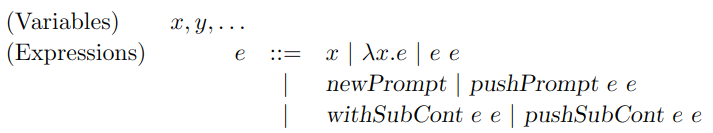
\includegraphics[width=0.75\linewidth]{figs/prompt-syntax}
%    \caption{Синтаксис $\lambda$-исчисления с примитивами для работы с продолжениями.}
%    \label{fig:prompt-syntax}
%\end{figure}
%
%\begin{figure}
%    \centering
%    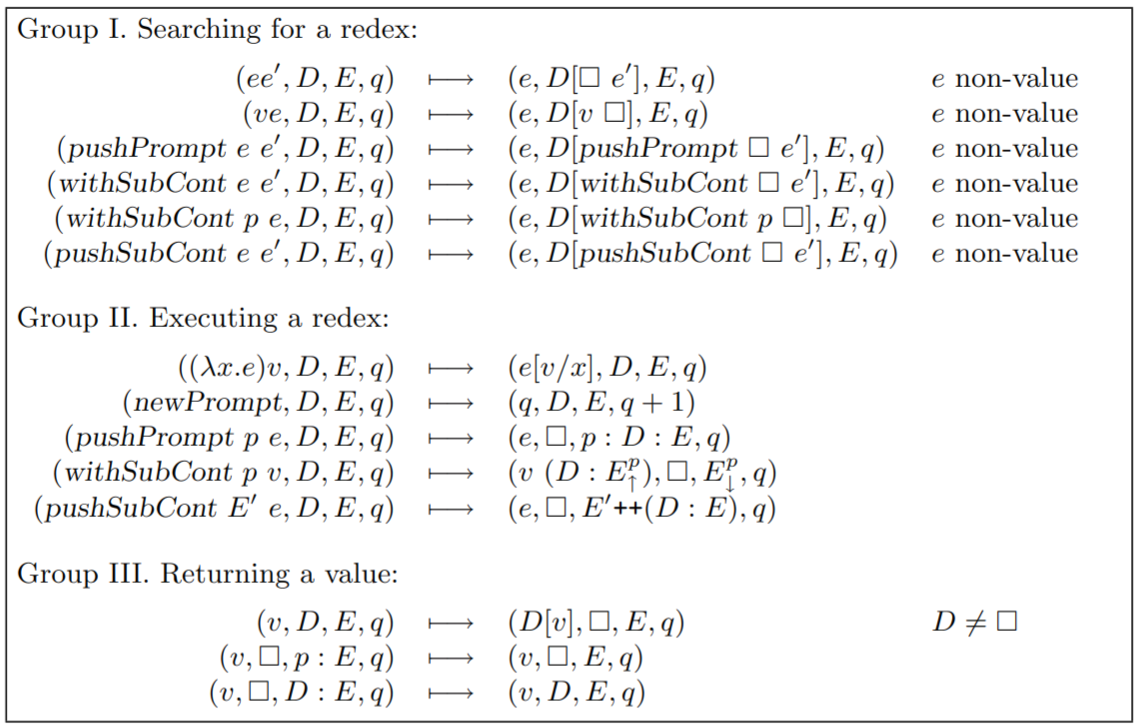
\includegraphics[width=0.8\textwidth]{figs/dc-operational}
%    \caption{Операционная семантика.}
%    \label{fig:dc-operational}
%\end{figure}
%
%\begin{itemize}
%    \item $newPrompt$ --- создаёт свежий идентификатор (метку) ограничения;
%    \item $pushPrompt \ap p \ap e$ --- устанавливает ограничение с меткой $p$ и исполняет выражение $e$;
%    \item $withSubCont\ap p\ap f$ --- захватывает частичное продолжение до ограничения с меткой $p$ и передаёт в функцию $f$, возвращает результат $f$ (рис.~\ref{fig:push-prompt});
%    \item $pushSubCont\ap k \ap v$ --- исполняет композицию текущего продолжения и $k$ на значении $v$.
%\end{itemize}
%
%\begin{figure}[h]
%    \centering
%    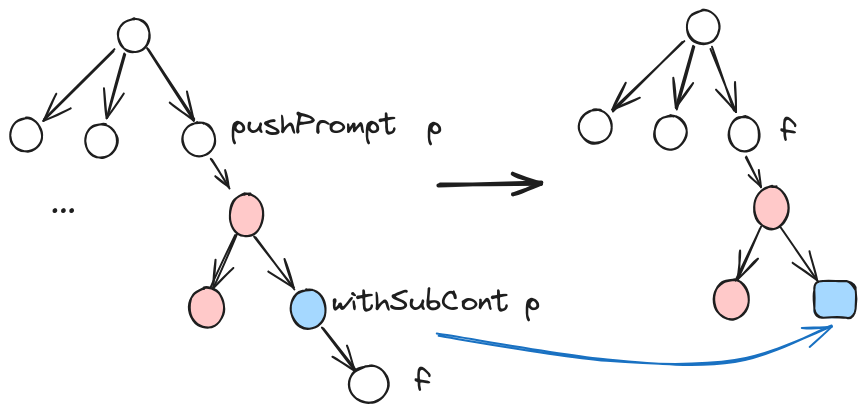
\includegraphics[width=0.7\linewidth]{figs/push-prompt}
%    \caption{Пример работы \texttt{withSubCont}.}
%    \label{fig:push-prompt}
%\end{figure}
%
%Операторы ограниченных продолжений легко понять как \vocab{resumable exceptions}, исключения, которые можно поймать, а программу возобновить с того места, где исключение было выброшено (с некоторым значением).
%Необычно то, что классические операторы ограниченных продолжений принимают код, работающий с частичным продолжением в месте ``кидания исключения'', а не в месте ``поимки''.
%То есть блок обработки пишется не с \mintinline{kotlin}|catch|, а с \mintinline{kotlin}|throw|:
%
%\begin{gather*}ч
%    E_1[withSubCont \ap p \ap \{E_2[pushSubCont \ap f]\}] \to E_1[f \ap E_2]
%    \\
%    E_1[catch\{E_2[throw \ap v], f\}] \to E_1[f \ap v \ap (\lambda x\ldotp E_2[x])]
%\end{gather*}
%
%\begin{figure}[h]
%    \centering
%    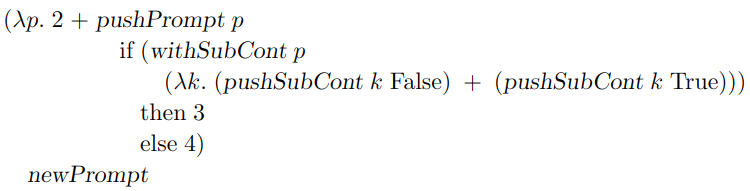
\includegraphics[width=0.8\linewidth]{figs/dc-example}
%    \caption{Пример выражения (результат --- $9$).}
%    \label{fig:dc-example}
%\end{figure}
%
%\begin{task}
%    Поредуцируйте пример рис.~\ref{fig:dc-example}.
%\end{task}
%
%Остальные операторы более-менее выражаются через обсуждённые нами.
%Существует классификаций операторов по признакам --- включает ли захватываемое частичное продолжение ограничение и оставляет ли его за собой~\cite{dyvbig2007monadic}.
%
%%\subsubsection{Реализация ограниченных продолжений}
%
%%\begin{task}
%%    Что изменится в реализации, если продолжения должны быть multi-shot?
%%\end{task}
%
%%\cite{mcbride2001derivative, huet1997zipper, ager2003functional}
%
%% todo in paper
%
%%\subsubsection{State machine}
%
%% todo Cont is for delimited continuations
%
%% todo
%
%%\subsubsection{Continuios stack}
%
%% todo
%
%%\subsubsection{Segmented stack}
%
%% todo
%
%% todo in haskell
%
%%\subsection{Использование продолжений}
%
%% todo trampolining
%
%% todo difference lists
%
%% todo lens
%
%% todo CPS интерпретаторы, переходы
%
%% todo корутины
%
%% todo генераторы
%
%% todo эффекты
%
%% todo transducers, pipelines and internal iteration
%
%% todo CEKT
%
%% todo continuation semantics
%
%% todo continuations and operating systems
%
%% todo single-shot/multi-shot
%
%% todo codensity
%
%% todo problems with continuations: typing and resources
%
%% todo implementing while & break
%
%% todo control operator, runtime наизнанку
%
%% todo sicp
%
%% todo CPS трансформация интерпретаторов
%
%% todo SPJ compiling without continuations
%
%% todo The Essence of Compiling with Continuations
%
%% todo calculating correct compilers
%
%% todo reference to best refactoring https://www.pathsensitive.com/2019/07/the-best-refactoring-youve-never-heard.html
%
%% todo game semantics from Carl's slides
%
%% todo STG machine and lazyness
%
%% todo http://www.serpentine.com/blog/2011/02/25/cps-is-great-cps-is-terrible/
%
%% todo https://www.joachim-breitner.de/blog/778-Don%E2%80%99t_think,_just_defunctionalize

% todo реализация продолжений

% todo семантика редукционных контекстов
